\climbingarea{South Freeport Coffin Area}{%
    \climbheader{This is in Freeport..}{This is public access Land Trust land.}{Park at the Pine St/South Freeport Roard intersection pullout and walk back up Pine St 200 ft.}{The area is often wet, but The Coffin boulder stays dry.}
    \climbingarea{The Coffin Boulder}{The Coffin Boulder is pretty cool.}{%
        % This is a comment
        % the syntax of \boulderproblem is:
        % \boulderproblem[number of stars]{Name}{Grade}{Description}{Height}{FA}
        \begin{minipage}{\linewidth}%
          \centering
          % This particular file is likely marked as "rotated" in the EXIF data, which LaTeX ignores...so we have to manually roate it here with the "angle" setting.
          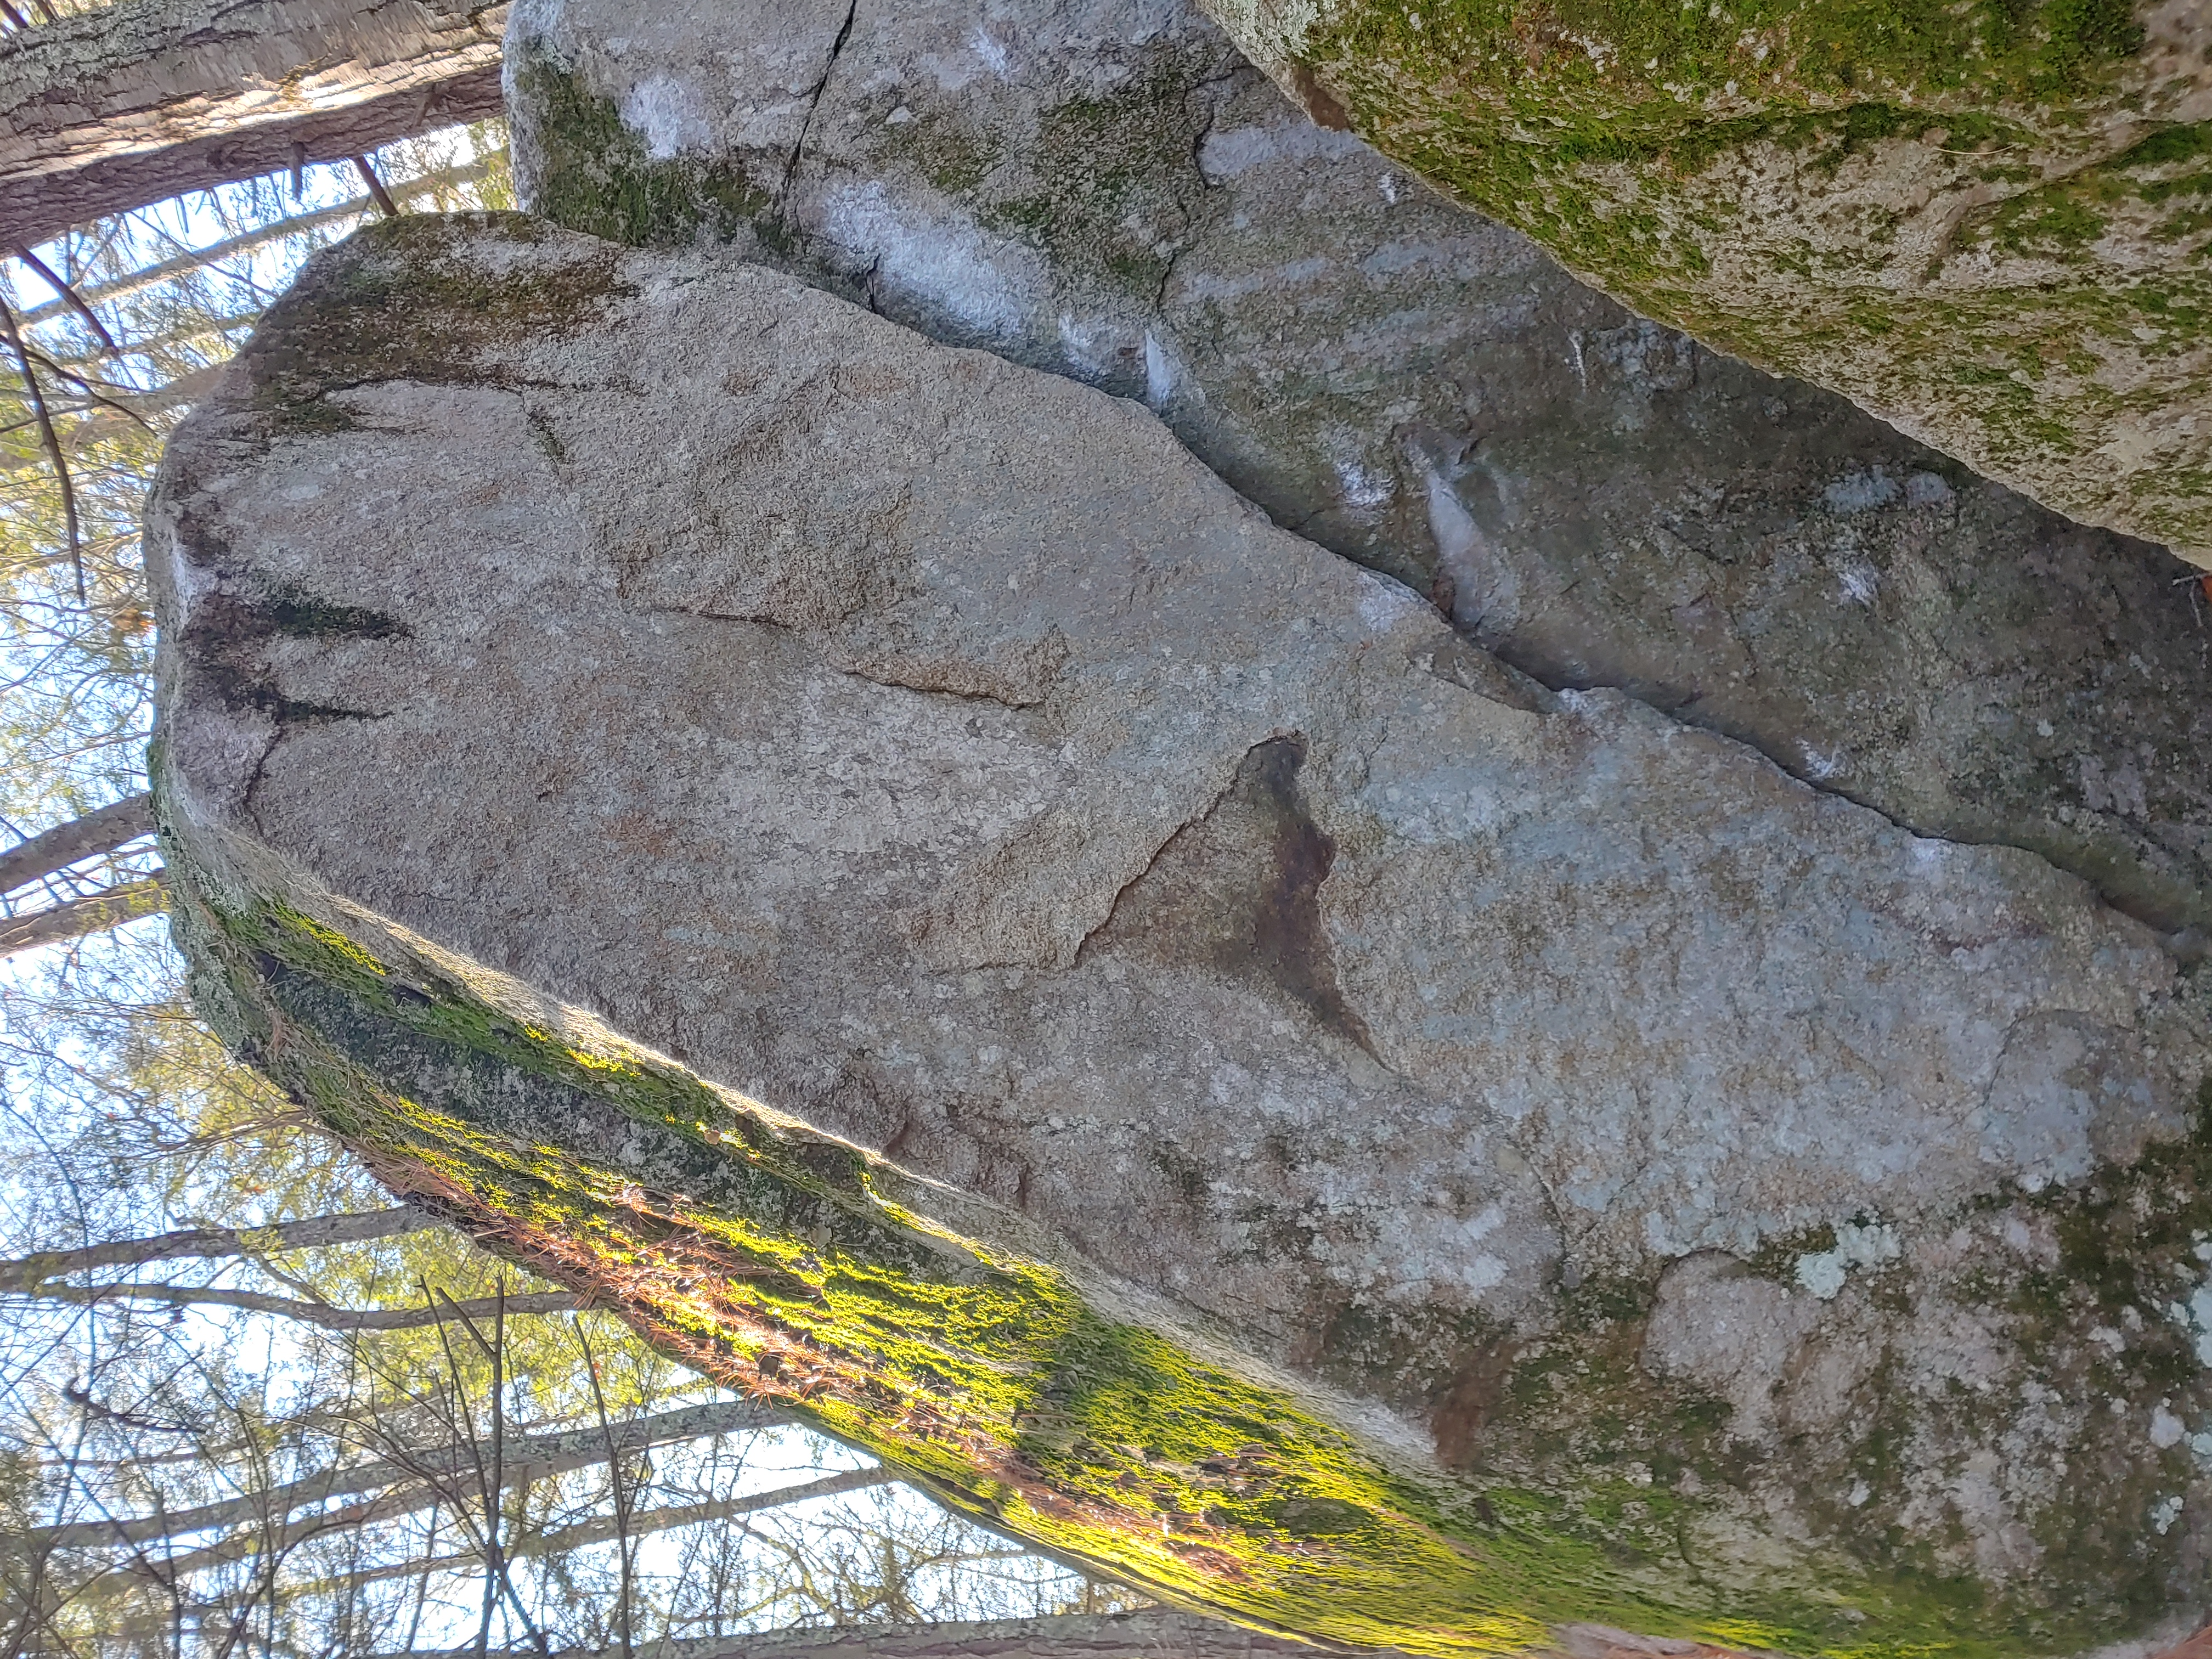
\includegraphics[angle=270,width=\linewidth]{1201251115_HDR.jpg}
          \captionof{figure}{The Coffin V8/9}
        \end{minipage}
        \boulderproblem[4]{The Coffin}{V8/9}{Sit-start with hands on either arete with thumbcatch. Climb up the prow with compression, topping out to the left..}{10}{Ben Yunker?}
        \boulderproblem[4]{Podule}{V6}{Sit-start with hands on the right side of sloper cracks. Climb up and left on rough slopers.}{10}{unknown}
    }
}{}
